سه شبکه‌ی مجزا تعریف شده است. برنامه‌ی جاوا فقط در \lr{edge-net} و \lr{redis-net} است و \lr{helper} فقط در \lr{helper-net}؛ بنابراین این دو {هیچ شبکه‌ی مشترکی ندارند} و تنها مسیر ممکن از جاوا به \lr{helper}، عبور از \lr{nginx} است که تنها عضو مشترک \lr{edge-net} و \lr{helper-net} است. این‌گونه شرط انجینکس حتما باید بین برنامه‌ی جاوا و آن سرویس باشد با {توپولوژی} تضمین می‌شود، نه با قرارداد.

\begin{center}
\begin{tabular}{|l|l|}
\hline
{محدودیت} & {راه‌حل} \\
\hline
فقط برنامه‌ی جاوا \lr{port mapping} داشته باشد & کلید \lr{ports} فقط زیر سرویس \lr{app} آمده است \\
\hline
کلمه‌ی \lr{environment} استفاده نشود & متغیرها از طریق \lr{env\_file} تزریق می‌شوند \\
\hline
\lr{nginx} بین جاوا و سرویس کمکی & جداسازی شبکه‌ها \\
\hline
نیاز به \lr{Redis} در زمان بالا آمدن & \lr{depends\_on} با شرط \lr{service\_healthy} \\
\hline
\end{tabular}
\end{center}

\lr{docker-compose.yaml}:

\begin{lstlisting}[language=Yaml]
name: ${COMPOSE_PROJECT_NAME:-ms-hw5-compose}

services:
  redis:
    image: ${REDIS_IMAGE}
    container_name: hw5-redis
    command: ["redis-server", "--save", "60", "1", "--loglevel", "warning"]
    volumes: [redis-data:/data]
    networks: [redis-net]
    healthcheck:
      test: ["CMD", "redis-cli", "ping"]
      interval: 5s
      retries: 10

  helper:
    build: { context: ./helper, dockerfile: Dockerfile }
    image: ${HELPER_IMAGE}
    container_name: hw5-helper
    networks: [helper-net]          # no ports: reachable only from nginx
    healthcheck:
      test: ["CMD", "python", "-c",
             "import urllib.request; urllib.request.urlopen('http://127.0.0.1:9090/helper').read()"]
      interval: 5s
      retries: 10

  nginx:
    image: ${NGINX_IMAGE}
    container_name: hw5-nginx
    volumes: ["./nginx.conf:/etc/nginx/nginx.conf:ro"]
    networks: [edge-net, helper-net]   # the only member of both networks
    depends_on:
      helper: { condition: service_healthy }
    healthcheck:
      test: ["CMD", "wget", "--spider", "-q", "http://127.0.0.1/healthz"]
      interval: 5s
      retries: 10

  app:
    image: ${APP_IMAGE}
    container_name: hw5-composeprac
    env_file:
      - ./env/app.env        # STUDENTID, HELPER_BASE_URL
      - ./env/redis.env      # REDIS_HOST, REDIS_PORT
    ports: ["${APP_PORT}:8080"]
    networks: [edge-net, redis-net]
    depends_on:
      redis: { condition: service_healthy }
      nginx: { condition: service_healthy }

networks:
  edge-net:   { driver: bridge }
  redis-net:  { driver: bridge, internal: true }
  helper-net: { driver: bridge, internal: true }

volumes:
  redis-data:
\end{lstlisting}

فایل‌های محیطی:

\begin{lstlisting}[language=bash]
# env/app.env                      # env/redis.env
STUDENTID=401105561                REDIS_HOST=redis
HELPER_BASE_URL=http://nginx:80    REDIS_PORT=6379
\end{lstlisting}

 \lr{nginx.conf}:

\begin{lstlisting}[language=Nginx]
worker_processes auto;
events { worker_connections 1024; }

http {
    include       /etc/nginx/mime.types;
    default_type  application/json;
    log_format proxy '$remote_addr -> $upstream_addr "$request" '
                     'status=$status upstream_status=$upstream_status';
    access_log /var/log/nginx/access.log proxy;
    server_tokens off;

    resolver 127.0.0.11 valid=10s ipv6=off;   # docker embedded DNS

    upstream helper_backend {
        server helper:9090;
        keepalive 16;
    }

    server {
        listen 80;
        server_name _;

        # the only endpoint the java app calls: GET ${HELPER_BASE_URL}/helper
        location = /helper {
            proxy_pass         http://helper_backend/helper;
            proxy_http_version 1.1;
            proxy_set_header   Connection "";
            proxy_set_header   Host              $host;
            proxy_set_header   X-Forwarded-For   $proxy_add_x_forwarded_for;
            proxy_connect_timeout 3s;
            proxy_read_timeout    10s;
        }

        location = /healthz { access_log off; return 200 '{"status":"ok"}\n'; }
        location /          { return 404 '{"error":"not found"}\n'; }
    }
}
\end{lstlisting}

سرویس کمکی هم با یک \lr{Dockerfile} کوچک روی \lr{python:3.12-alpine} که \lr{EXPOSE 9090} در آن فقط مستندسازی است و هیچ پورتی روی میزبان باز نمی‌کند.

 اجرا و دو خط لاگ:

\begin{lstlisting}[language=bash]
docker build -t composeprac compose-challenge
docker compose up -d
curl -s -X POST http://localhost:8080/call-me
docker compose logs app
\end{lstlisting}

\begin{figure}[H]
\centering
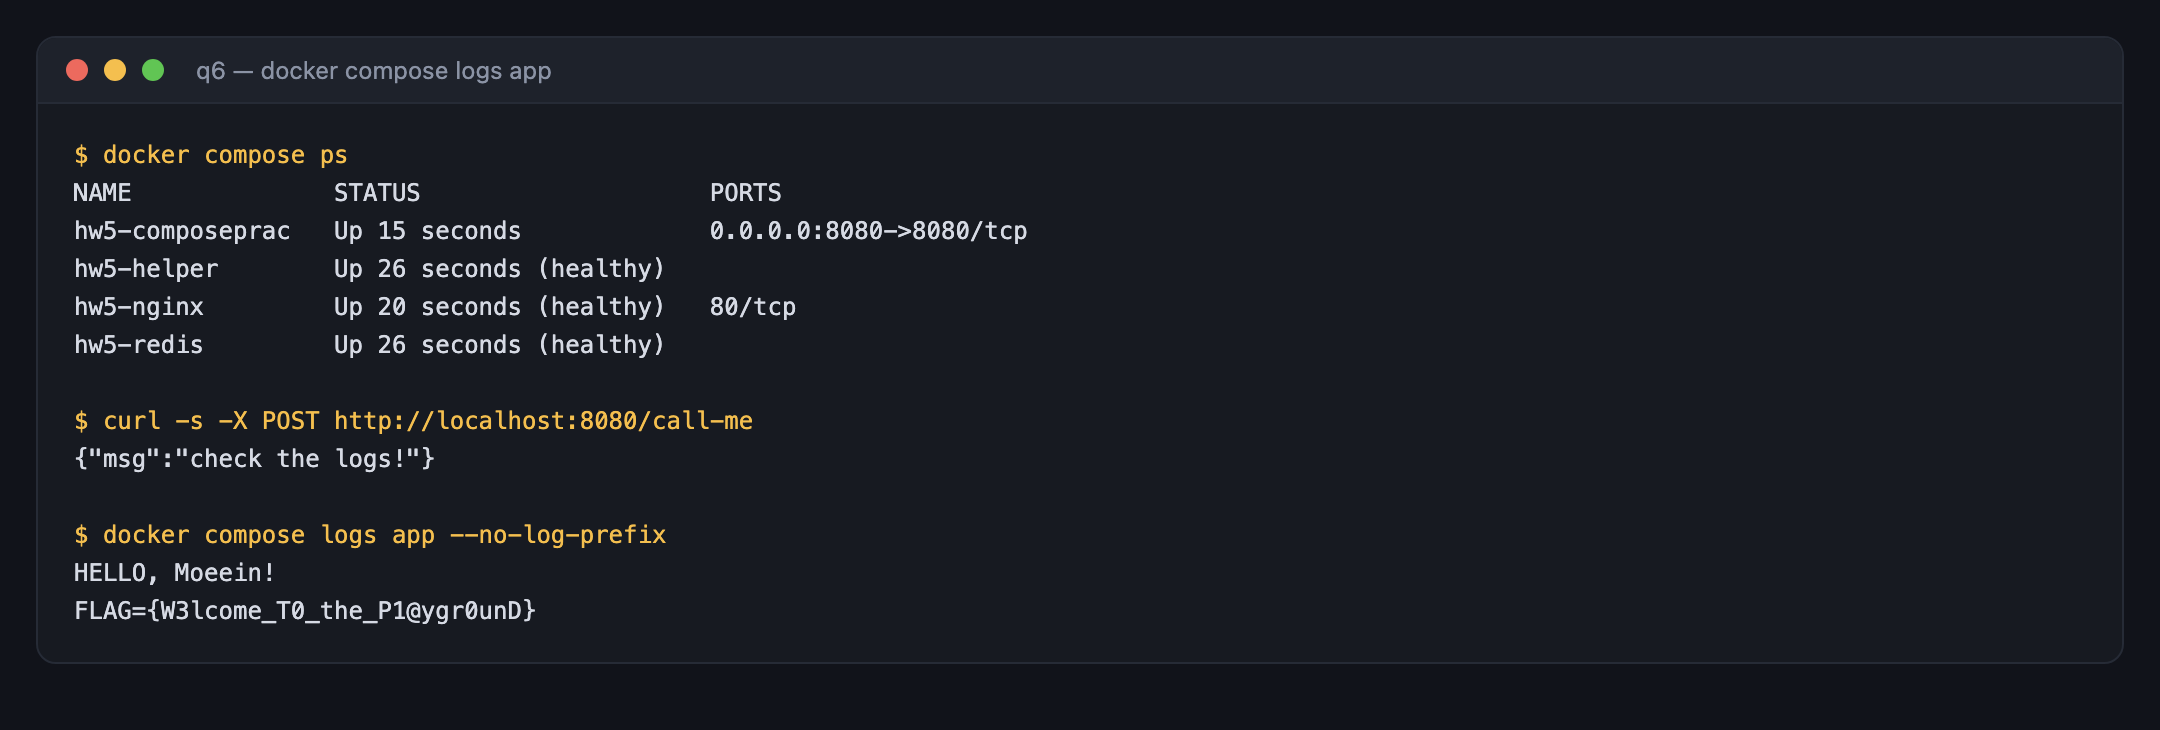
\includegraphics[width=0.94\textwidth]{figs/q6-run.png}
\caption{دو خط لاگ خواسته‌شده: پیام شخصی و فلگ.}
\end{figure}

دو خط لاگ به‌دست‌آمده:

\begin{lstlisting}[language={},basicstyle=\ttfamily\small,numbers=none]
HELLO, Moeein!
FLAG={W3lcome_T0_the_P1@ygr0unD}
\end{lstlisting}

برای اینکه نشان دهیم \lr{nginx} واقعا در مسیر است (و نه صرفا کنار آن)، از یک کانتینر روی \lr{edge-net}  یک‌بار مستقیم به \lr{helper} و یک‌بار از طریق \lr{nginx} درخواست زده شد:

\begin{figure}[H]
\centering
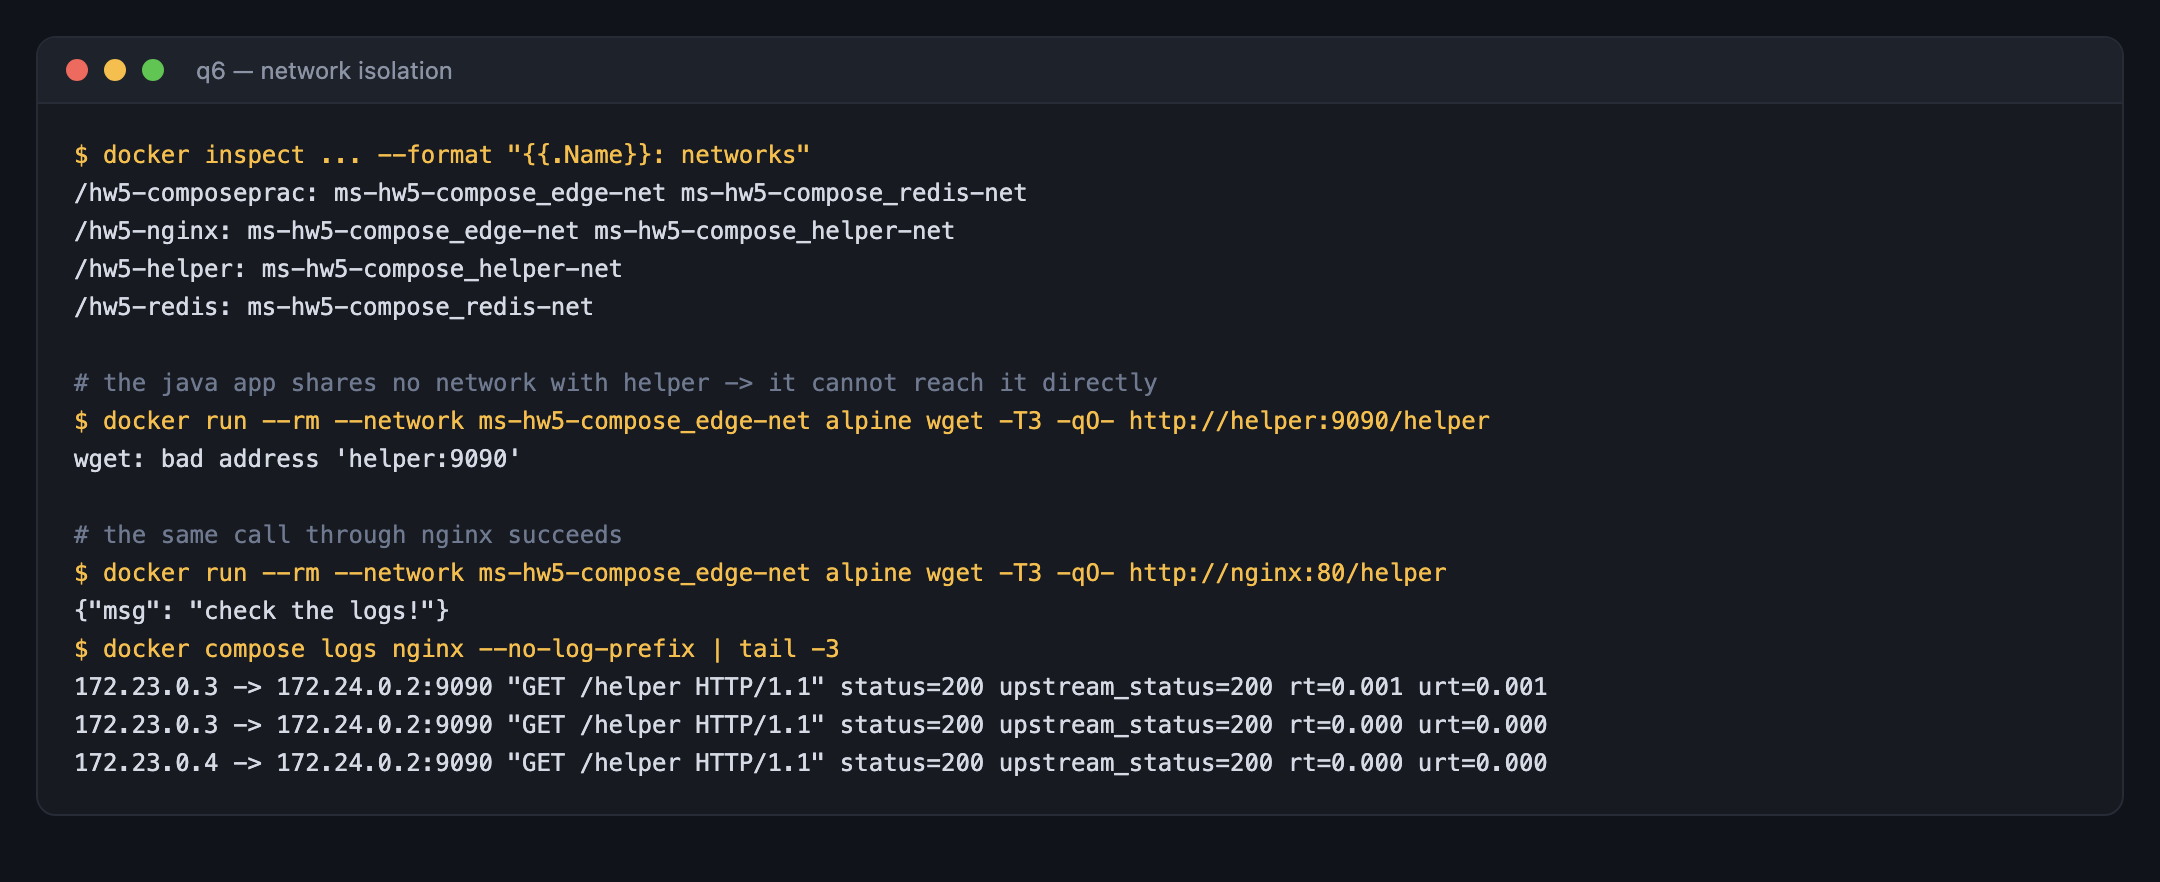
\includegraphics[width=0.94\textwidth]{figs/q6-net.png}
\caption{از شبکه‌ی برنامه‌ی جاوا، نام \lr{helper} اصلا قابل \lr{resolve} نیست؛ اما همان درخواست از مسیر \lr{nginx} پاسخ می‌گیرد و در \lr{access log} انجینکس ثبت می‌شود.}
\end{figure}

\subsubsection*{استفاده‌ی داکر کامپوز از فایل‌های \lr{env}}

کامپوز دو سازوکار کاملا متفاوت دارد که اغلب با هم اشتباه گرفته می‌شوند:

{۱. فایل \lr{.env} کنار \lr{docker-compose.yaml}.} این فایل به‌صورت خودکار خوانده می‌شود و مقادیرش {درون خود فایل کامپوز} جای‌گذاری می‌شود؛ یعنی روی نام ایمیج، شماره‌ی پورت، نام پروژه و هر جای دیگری که \lr{\$\{VAR\}} نوشته شده اثر می‌گذارد. این متغیرها به‌خودی‌خود وارد کانتینر {نمی‌شوند}. در این تمرین \lr{.env} شامل \lr{APP\_IMAGE}، \lr{APP\_PORT}، \lr{REDIS\_IMAGE} و \lr{NGINX\_IMAGE} است.

{۲. کلید \lr{env\_file} زیر یک سرویس.} محتوای این فایل‌ها به‌عنوان متغیر محیطی {داخل همان کانتینر} تزریق می‌شود و در فایل کامپوز قابل استفاده نیست. اینجا \lr{env/app.env} و \lr{env/redis.env} دقیقا همان چهار متغیر مورد نیاز برنامه‌ی جاوا را می‌دهند.

نکات کاربردی:
\begin{itemize}
	\item ترتیب اولویت از کم به زیاد: مقدار پیش‌فرض در \lr{Dockerfile} (\lr{ENV}) $\leftarrow$ \lr{env\_file} $\leftarrow$ کلید \lr{environment} $\leftarrow$ متغیر پاس‌داده‌شده در خط فرمان.
	\item چند \lr{env\_file} مجاز است و در تعارض، فایل بعدی برنده است.
	\item فایل \lr{env\_file} با \lr{shell} تفسیر نمی‌شود: نه بسط متغیر دارد، نه \lr{export} می‌خواهد و کوتیشن‌ها بخشی از مقدار محسوب می‌شوند.
	\item مسیر \lr{.env} پیش‌فرض کنار فایل کامپوز است و با \lr{--env-file} قابل تعویض است؛ الگوی رایج داشتن \lr{.env.example} در مخزن و نگه داشتن \lr{.env} واقعی بیرون از گیت است.
\end{itemize}

\subsubsection*{ انواع \lr{Network} در داکر}

\begin{center}
\begin{tabular}{|l|l|}
\hline
{درایور} & {توضیح} \\
\hline
\lr{bridge} & شبکه‌ی خصوصی روی یک میزبان. شبکه‌ی \lr{bridge} کاربرساخته \lr{DNS} داخلی \\
 & دارد و کانتینرها با نام یکدیگر را می‌بینند (برخلاف \lr{bridge} پیش‌فرض). \\
\hline
\lr{host} & کانتینر مستقیما از \lr{network namespace} میزبان استفاده می‌کند؛ جداسازی شبکه ندارد \\
 & و \lr{port mapping} بی‌معناست. برای کارایی بالا یا کشف سرویس در سطح میزبان. \\
\hline
\lr{none} & هیچ رابط شبکه‌ای جز \lr{loopback}؛ برای کارهای کاملا ایزوله و پردازش داده‌ی نامطمئن. \\
\hline
\lr{overlay} & شبکه‌ی چندمیزبانه روی \lr{Swarm}؛ کانتینرهای ماشین‌های مختلف را در یک \lr{L2} \\
 & مجازی قرار می‌دهد و رمزنگاری اختیاری دارد. \\
\hline
\lr{macvlan} & به کانتینر آدرس \lr{MAC} و \lr{IP} مستقل روی شبکه‌ی فیزیکی می‌دهد؛ برای \\
 & سامانه‌های قدیمی که باید مستقیما در شبکه‌ی سازمان دیده شوند. \\
\hline
\lr{ipvlan} & مشابه \lr{macvlan} اما با اشتراک \lr{MAC}؛ مناسب جایی که سوییچ محدودیت \lr{MAC} دارد. \\
\hline
\end{tabular}
\end{center}

دو صفت مهم و مستقل از درایور:
\begin{itemize}
	\item {\lr{internal: true}}: شبکه به دنیای بیرون مسیر ندارد. در این تمرین \lr{redis-net} و \lr{helper-net} از این نوع‌اند؛ یعنی حتی اگر کسی در آن کانتینرها کد دلخواه اجرا کند، خروجی به اینترنت ندارد.
	\item {\lr{external: true}}: شبکه از قبل بیرون از کامپوز ساخته شده و مدیریتش با کامپوز نیست (توضیح سؤال ۱).
\end{itemize}
